\chapter{Coding Agents and AI for Vulnerability Detection}
\label{chap:lec05_coding_agents_vulnerability_detection}
\section{本讲学习目标}
\begin{itemize}
\item 理解 coding agent 的定义为何强调多轮工具使用和 environment feedback。
\item 区分 dynamic control 与 procedural control 两类 coding-agent 设计。
\item 理解 security tasks 为什么要求交互式工具、sandbox 和强验证。
\item 看懂 Big Sleep 如何把真实漏洞研究 framing 成 variant analysis workflow。
\end{itemize}

\section{为什么 evaluator 先于 architecture}
Sutton 开头最重要的技术观点，其实不是某个 agent loop，而是 evaluator 决定设计。早期代码生成 benchmark 如 HumanEval 和 MBPP 强调 pass@k：给定 prompt，采样若干程序，看其中是否有正确答案。这类 evaluator 在 2021 年非常有用，因为难度适中、不易泄漏、能推动模型进步；但到 2025 年，它们已经太容易、测试用例太少、泄漏也太严重，很难再指导 agent 设计。

\begin{figure}[H]
\centering
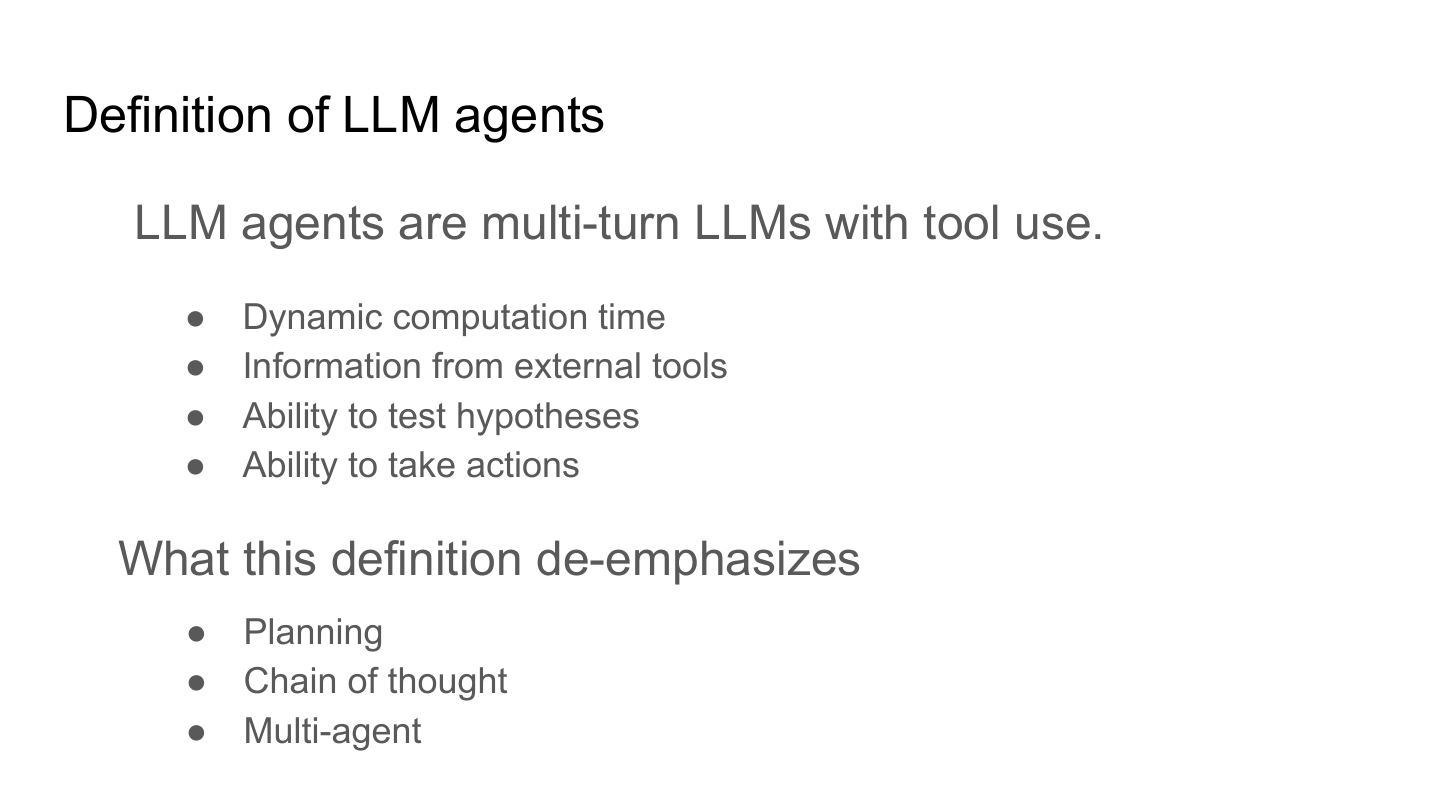
\includegraphics[width=0.78\textwidth]{../lectures/lec05_coding_agents_vulnerability_detection/figures/lec05_fig_001.png}
\caption{Sutton 的 LLM agent 定义：多轮、带工具、可测试假设、可采取行动。}
\end{figure}

\begin{figure}[H]
\centering
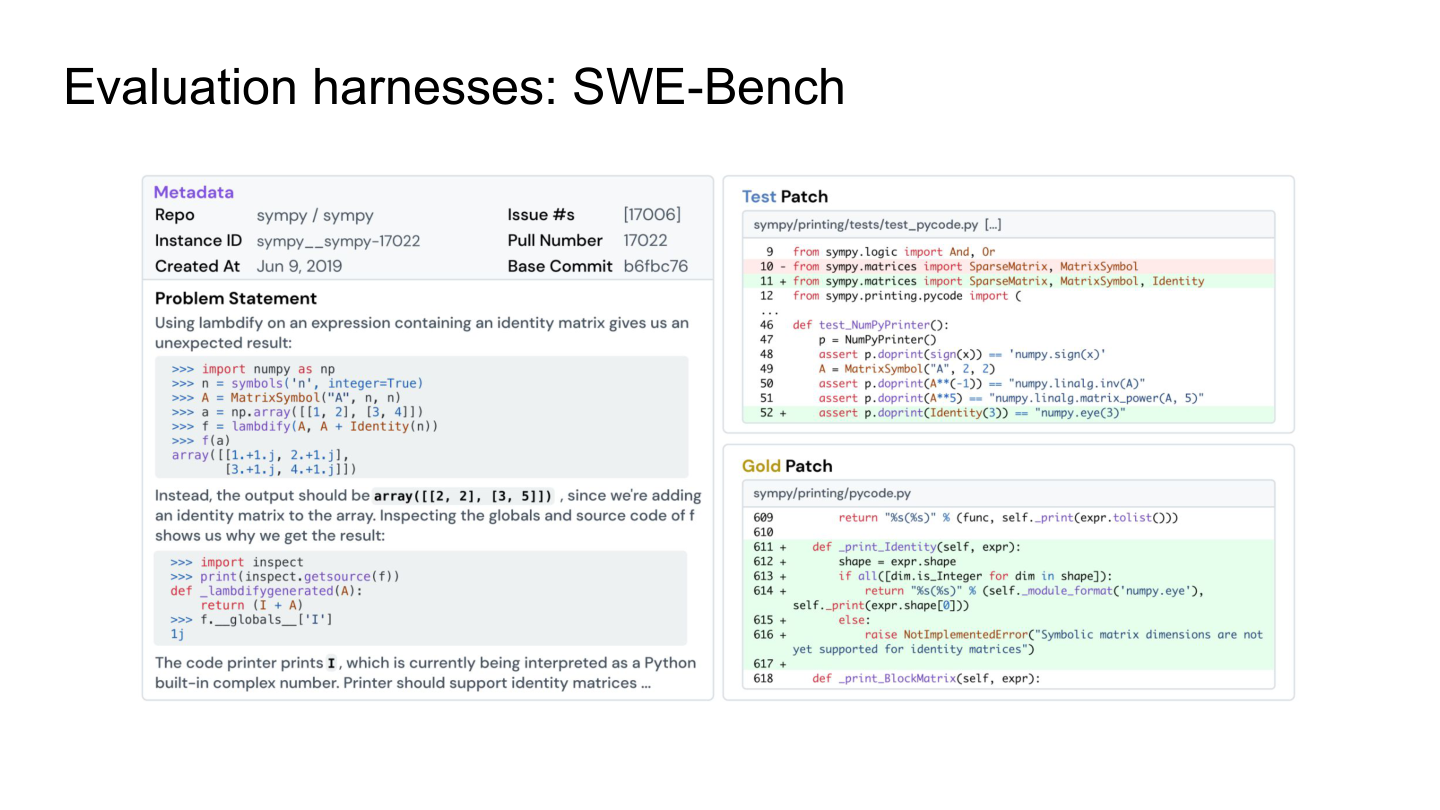
\includegraphics[width=0.8\textwidth]{../lectures/lec05_coding_agents_vulnerability_detection/figures/lec05_fig_002.png}
\caption{SWE-Bench 这类 evaluator 改变了 coding agent 设计方向：系统不再只做单函数合成，而是要处理真实仓库中的定位、修改和验证。}
\end{figure}

\[
\\operatorname{pass@k} = 1 - \\frac{{n-c \\choose k}}{{n \\choose k}}
\]

这个公式对应 lecture 中对 pass@k 的统计解释。$n$ 是总样本数，$c$ 是其中正确样本数，$k$ 表示允许查看或执行的样本数。它的工程意义在于：它既衡量正确率，也间接衡量样本多样性。但 Sutton 同时提醒，pass@k 是否合理，还取决于它是否贴近真实产品使用方式。

\begin{knowledgebox}{本讲的第一原则}
如果 evaluator 不能代表真实工作流，agent architecture 很容易被优化到错误方向。也就是说，benchmark 不是测量工具而已，它会塑造你最终造出来的系统。
\end{knowledgebox}

\section{coding agent 的核心：控制流与工具接口}
\subsection{ReAct 与动态 tool-using agent}
Lecture 中的 SWE-Agent 是动态 coding agent 的代表。其基本思想很简单：LLM 根据当前 trajectory 提出下一步动作，系统运行工具，再把输出追加回 trajectory，直到成功、超时或失败。

\begin{figure}[H]
\centering
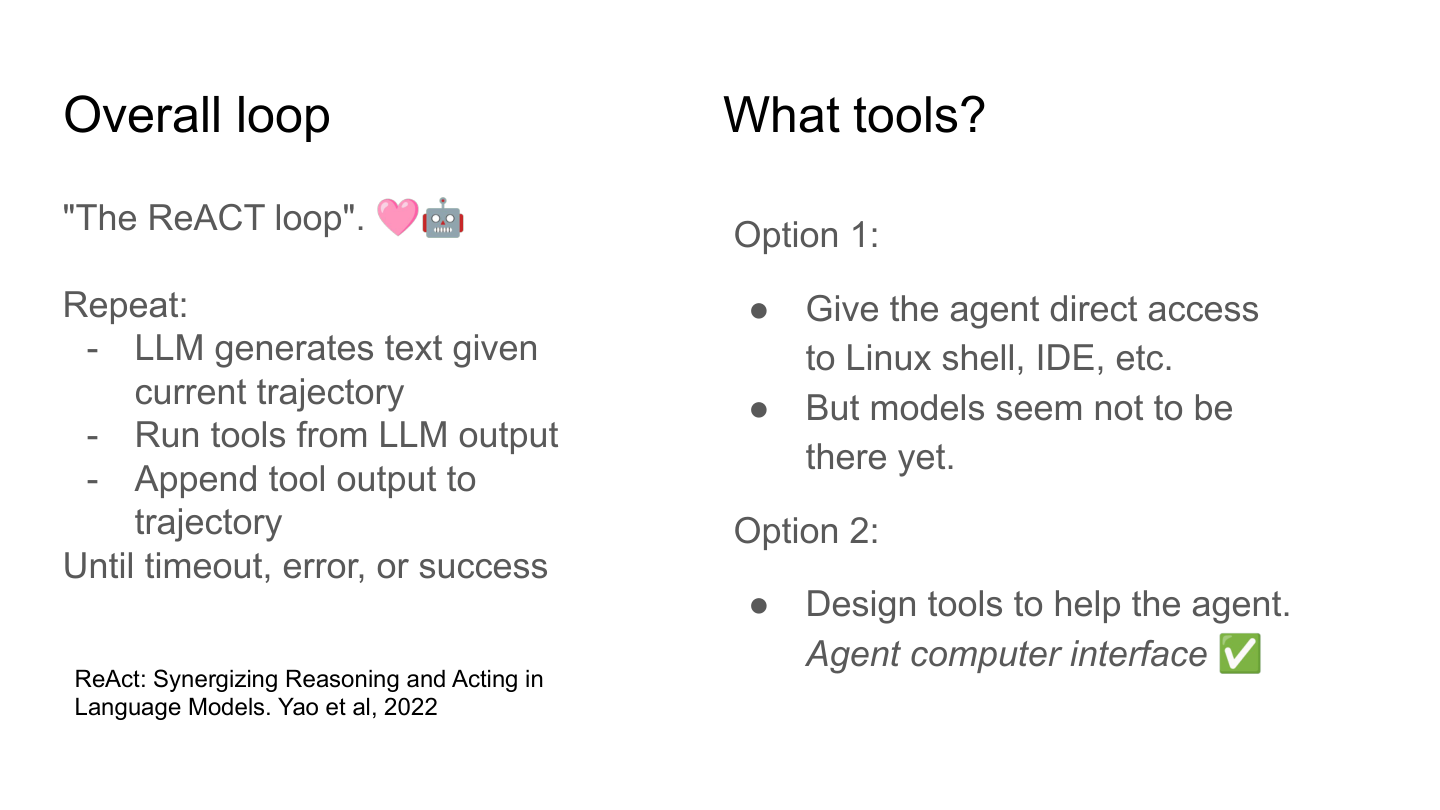
\includegraphics[width=0.76\textwidth]{../lectures/lec05_coding_agents_vulnerability_detection/figures/lec05_fig_003.png}
\caption{ReAct loop：thought/action/observation 的循环是 coding agent 最经典的最小控制结构。}
\end{figure}

\[
\\tau = (o_1, a_1, o_2, a_2, \\ldots), \\qquad \\max_{\\pi} \\mathbb{E}[R(\\tau)] \\ \\text{s.t.} \\ |\\tau| \\le B
\]

这个抽象表达了 lecture 对 agent trajectory 的理解：你优化的是整条轨迹 $\\tau$ 的成功率，而不是单次文本输出；同时轨迹长度受预算 $B$ 约束。这比“让模型多想一点”更具体，因为每一步都有工具成本、噪声和延迟。

\begin{lstlisting}
trajectory = []
while not done and budget_left():
    action = llm(trajectory)
    observation = run_tool(action)
    trajectory.append((action, observation))
\end{lstlisting}

Sutton 对 agent-computer interface 的要求很值得教材化记录：工具要简单、反馈要紧凑、动作空间要鼓励高信息密度而不是长篇废话、并且必须有 guardrails。这说明 agent intelligence 的相当一部分，其实来自 interface design。

\begin{figure}[H]
\centering
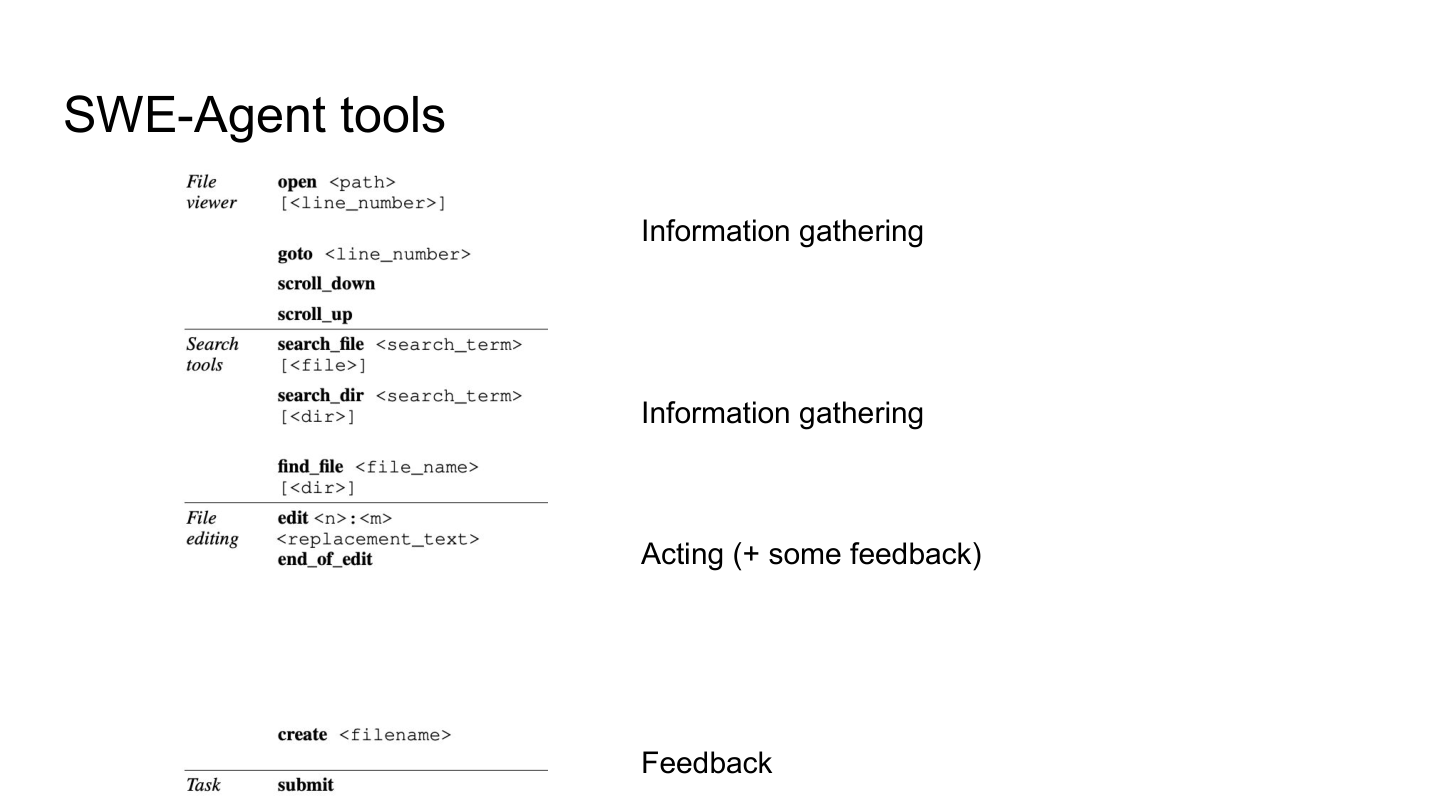
\includegraphics[width=0.82\textwidth]{../lectures/lec05_coding_agents_vulnerability_detection/figures/lec05_fig_004.png}
\caption{SWE-Agent 的工具层次：信息收集、行动和反馈构成闭环。}
\end{figure}

\subsection{Agentless、AutoCodeRover 与 procedural control}
Sutton 讲得非常清楚：并不是所有 coding task 都需要最高自由度的动态 agent。Agentless 和 AutoCodeRover 展示了一类 procedural control：先把大工作流写出来，例如 localization、patch generation、ranking，然后在局部节点调用模型。它们的价值是更稳定、更容易调试，也更容易把 test-time compute 投到确定的阶段上。

\begin{figure}[H]
\centering
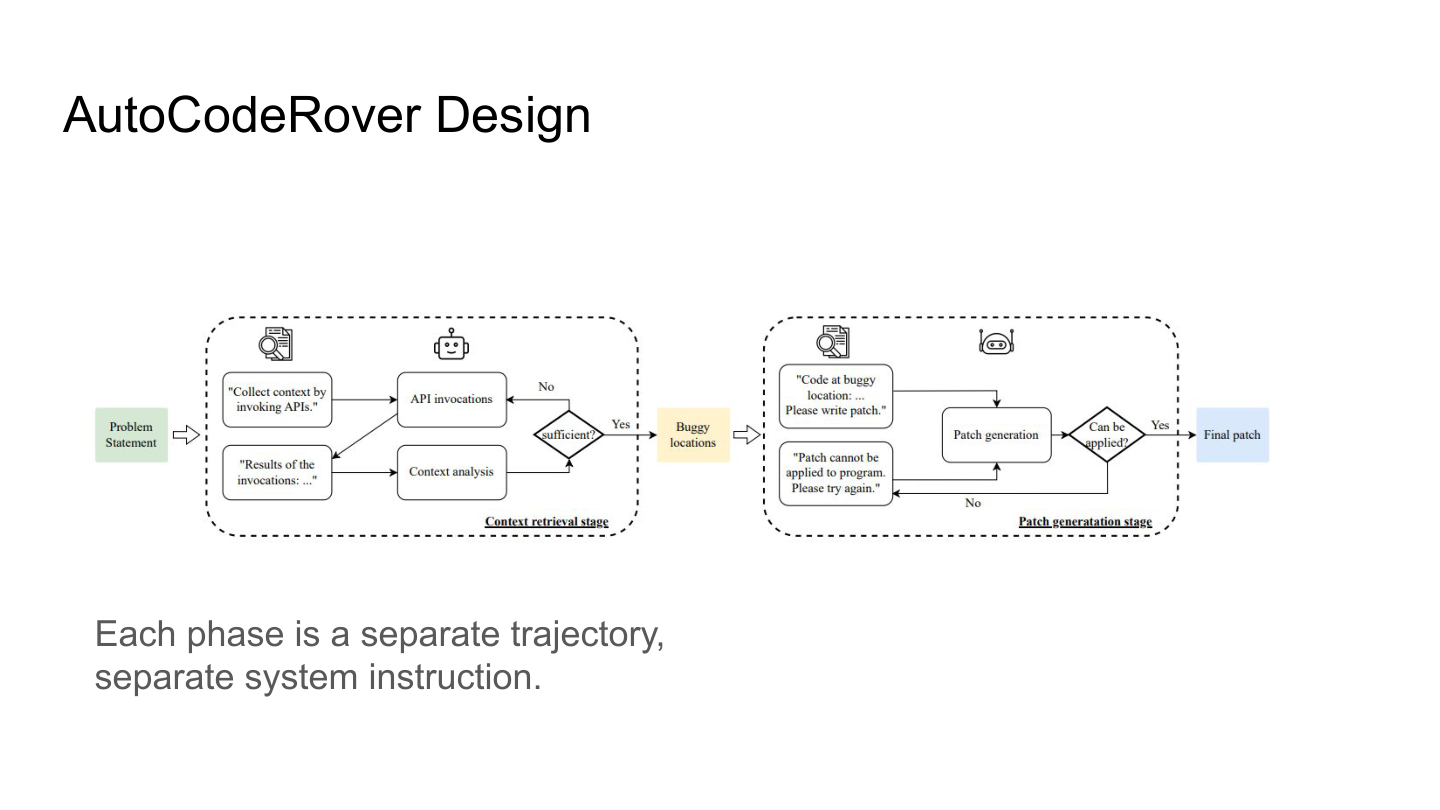
\includegraphics[width=0.76\textwidth]{../lectures/lec05_coding_agents_vulnerability_detection/figures/lec05_fig_005.png}
\caption{AutoCodeRover 的阶段式设计：每一阶段有独立 trajectory 和独立 instruction，是介于静态 pipeline 与完全动态 agent 之间的折中。}
\end{figure}

\begin{lstlisting}
files = localize_issue(repo, bug_report)
patches = synthesize_candidate_patches(files)
ranked = rerank_with_tests(patches)
return ranked[0]
\end{lstlisting}

这类设计解决的问题是可控性。若 workflow 本身相对固定，把控制流外移到显式 Python/状态机中，往往比把一切交给 LLM 更可靠。代价是探索能力受限，遇到奇怪错误时可能不如动态 agent 灵活。

\subsection{design space：真正要调的是哪几个旋钮}
Passerine 和 design-space slides 提供了一个很好的统一框架：你实际上在同时设计 tools、control flow、prompting/memory。它们彼此耦合。例如工具很多且噪声大时，过度动态的 agent 会反复迷路；任务很开放时，纯 procedural pipeline 又会过早锁死策略空间。

\begin{lstlisting}
design = {
  'tools': ['search', 'edit', 'execute', 'feedback'],
  'control_flow': ['procedural', 'state_machine', 'dynamic', 'tree_search'],
  'prompting': ['system role', 'phase instructions', 'memory']
}
\end{lstlisting}

\begin{importantbox}{dynamic 和 procedural 不是价值观之争}
Lecture 的真正问题是：test-time compute 应该放在哪。是让 agent 在单条轨迹里自由探索，还是把预算分配给更窄但更稳定的程序化阶段？这和第一讲、第四讲关于 test-time compute 的讨论直接相连。
\end{importantbox}

\section{从 coding tasks 到 security tasks}
安全任务与普通 coding tasks 的关键区别，不在于“代码更难”，而在于 evaluator 更硬、环境更复杂、验证更重要。CTF 任务要求 agent 理解协议、交互式程序、二进制、网络服务和 exploit 条件，很多时候单看源码根本不够。

\begin{figure}[H]
\centering
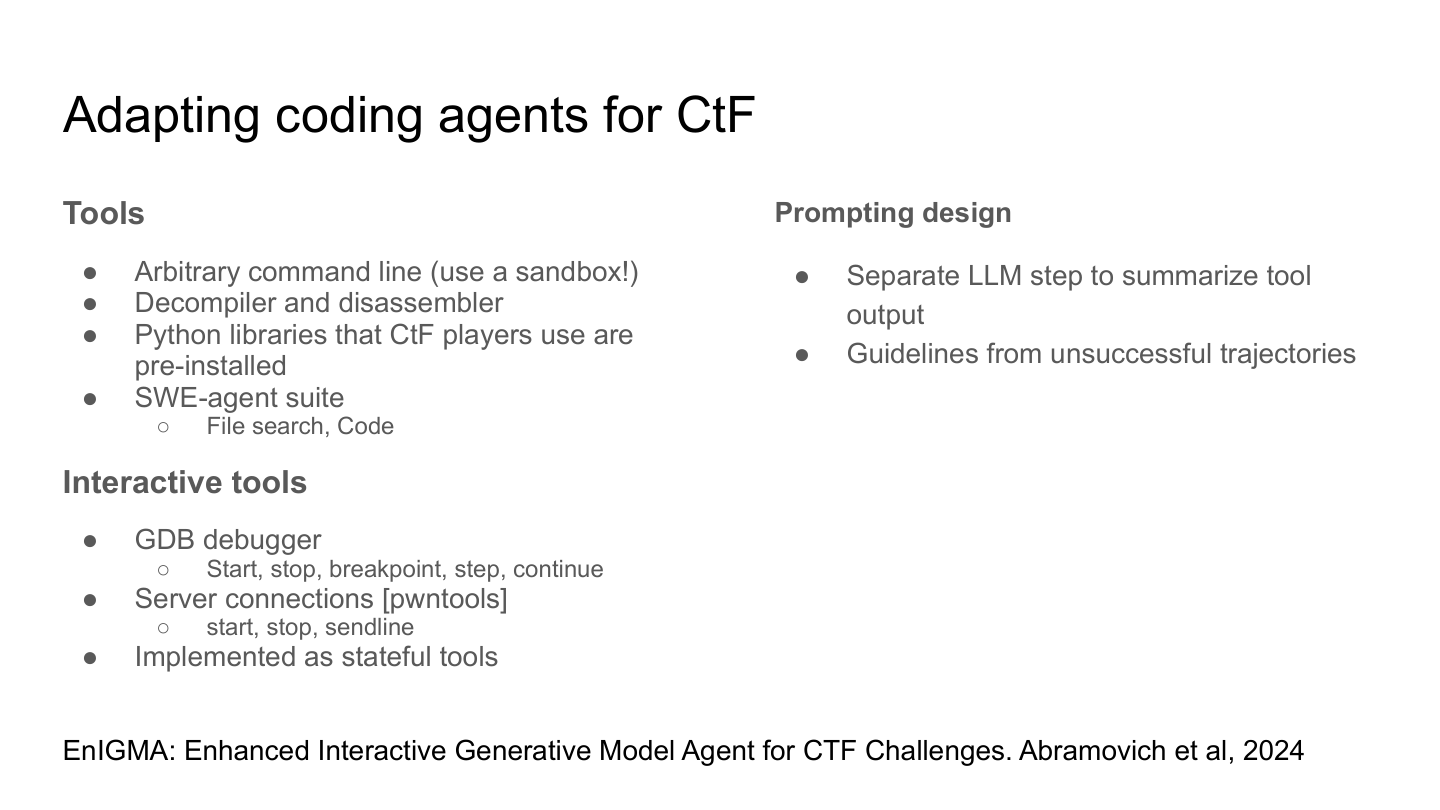
\includegraphics[width=0.8\textwidth]{../lectures/lec05_coding_agents_vulnerability_detection/figures/lec05_fig_006.png}
\caption{EnIGMA 的 interactive tools：debugger、server connection、shell 与 Python 工具让 agent 能进入安全问题真正的状态空间。}
\end{figure}

\begin{lstlisting}
while not solved:
    tool_call = lm.choose(['shell', 'debugger', 'server', 'python'])
    obs = execute(tool_call)
    update_context(obs)
    if flag_found(obs):
        break
\end{lstlisting}

《EnIGMA》reading 把 lecture 的直觉变成了证据：交互式工具显著提升了 security agents 在 CTF benchmark 上的表现。这说明安全 agent 不是普通 coding agent 加一句 “think like a hacker” 就能得到的；它需要完全不同的信息接口和验证接口。

但教材化地看，EnIGMA 的价值和边界都要同时看到。它证明 interactive tools 能显著改变 security-task performance，这一点非常重要；可它主要仍然是在 CTF-style environment 中验证方法。CTF 的好处是目标清晰、反馈直接、flag 导向明确，因此它非常适合回答“如果给 agent debugger、server connection 与 shell，会不会更强”。可它不自动回答另一个更难的问题：\textbf{这些能力能否稳定迁移到真实生产仓库中的长期漏洞研究？}

这正是 lecture 后半段转向 Big Sleep 的原因。Sutton 并不是否定 CTF benchmark，而是把它放在一个更大的 capability ladder 里：CTF 先证明工具接口有价值；真实仓库研究再检验 agent 能否在更稀疏、更含糊、更多上下文依赖的环境里发挥作用。

\section{漏洞检测：为什么“看起来像 bug”远远不够}
Slides 在漏洞检测部分很务实。一个 software vulnerability 不只是程序错误，而是具有安全含义的程序错误，例如 XSS、越界读写、SQL 注入、use-after-free 等。判断这类问题通常需要：
\begin{itemize}
\item 更大的全局上下文，而不是单个函数的局部文本。
\item 对输入约束、调用路径与 exploitability 的理解。
\item 来自执行、sanitizer、fuzzing 或其他分析器的验证信号。
\item 结合历史补丁和 CVE 语境做 variant analysis。
\end{itemize}

因此，普通编程 benchmark 上的高分并不自动转化为高质量 vulnerability detection。Sutton 专门把 NVD、AI Cyber Challenge、传统 fuzzing/static analysis 放进同一段，就是为了强调：安全 agent 应该与这些已有验证工具协作，而不是取代它们。

\section{Big Sleep：真实仓库中的 variant analysis agent}
Lecture 最关键的 case study 是 Big Sleep。它之所以重要，不仅因为它找到了真实世界漏洞，更因为它选择了一个更可信的任务 framing：variant analysis。也就是说，不让 agent 在无限开放的仓库空间里瞎逛，而是利用 recent commits、diffs、历史 bug patterns 作为 seed hint，围绕这些线索做针对性搜索。

\begin{figure}[H]
\centering
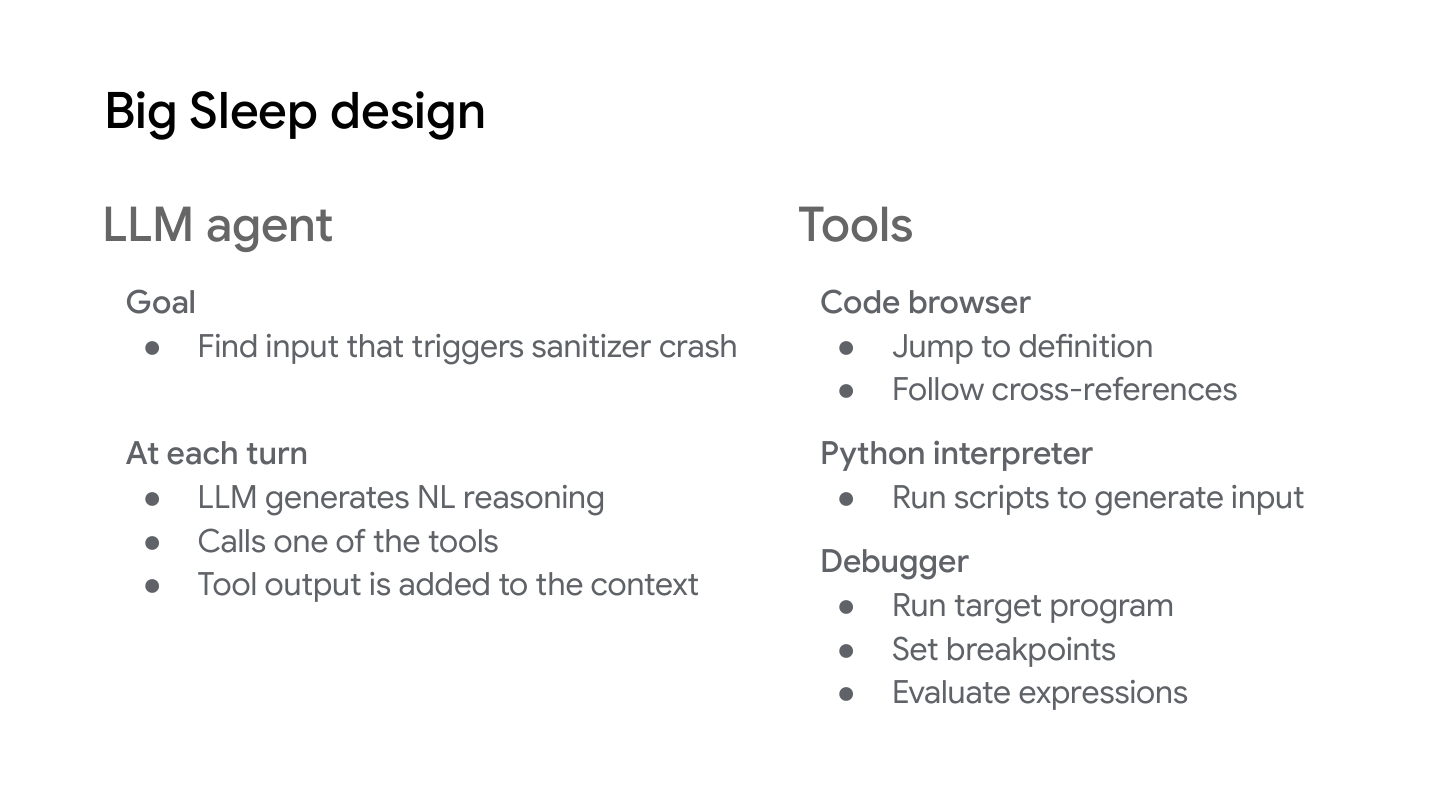
\includegraphics[width=0.8\textwidth]{../lectures/lec05_coding_agents_vulnerability_detection/figures/lec05_fig_007.png}
\caption{Big Sleep 的工作流：从代码浏览、到工具执行、到 hypothesis revision，核心是 tool-grounded variant analysis。}
\end{figure}

\[
\\max_{a_{1:T}} \\ \\Pr\\big[V(\\text{{repo}}, a_{1:T}) = 1 \\mid \\text{{seed hint}}\\big]
\]

这个抽象表达了 variant-analysis workflow 的本质：不是最大化“模型能否想出漏洞故事”，而是最大化在 seed hint 条件下，通过动作序列 $a_{1:T}$ 找到可被 verifier 证实的真实问题的概率。这里的 verifier 可以是 sanitizer crash、真实 exploit signal 或其它独立证据。

\begin{lstlisting}
for diff in recent_security_relevant_commits:
    hypothesis = llm.propose_variant(diff)
    trace = browse_repo_and_execute(hypothesis)
    if verifier(trace):
        report_vulnerability(trace)
\end{lstlisting}

Project Zero 的 Big Sleep 文章进一步说明了 lecture 没有完全展开的两点。第一，真实成果依赖 repository context 和 diff-aware prompting，而不是纯文本问答。第二，这项工作被明确放在防御者视角：在漏洞正式发布前发现并修补它，减少攻击者可利用窗口。

把《EnIGMA》和 Big Sleep 放在一起看，本讲其实给出了一条很清楚的 security-agent 递进路线：
\begin{itemize}
\item 先在 CTF 或 sandboxed challenge 中验证 \textbf{tool interface} 是否真的改善搜索与验证。
\item 再在真实仓库里使用 diff、recent commits、历史补丁模式等线索，把任务重构成更可控的 \textbf{variant analysis}。
\item 最后才讨论更开放的 defensive deployment，包括 provenance、sandbox、日志、权限控制和 human escalation。
\end{itemize}

这样看，Big Sleep 不是“模型忽然更聪明了”的故事，而是 lecture 全程都在强调的同一个原则：\textbf{高风险 agent 的价值来自 workflow grounding，而不是语言流畅性。}

\begin{figure}[H]
\centering
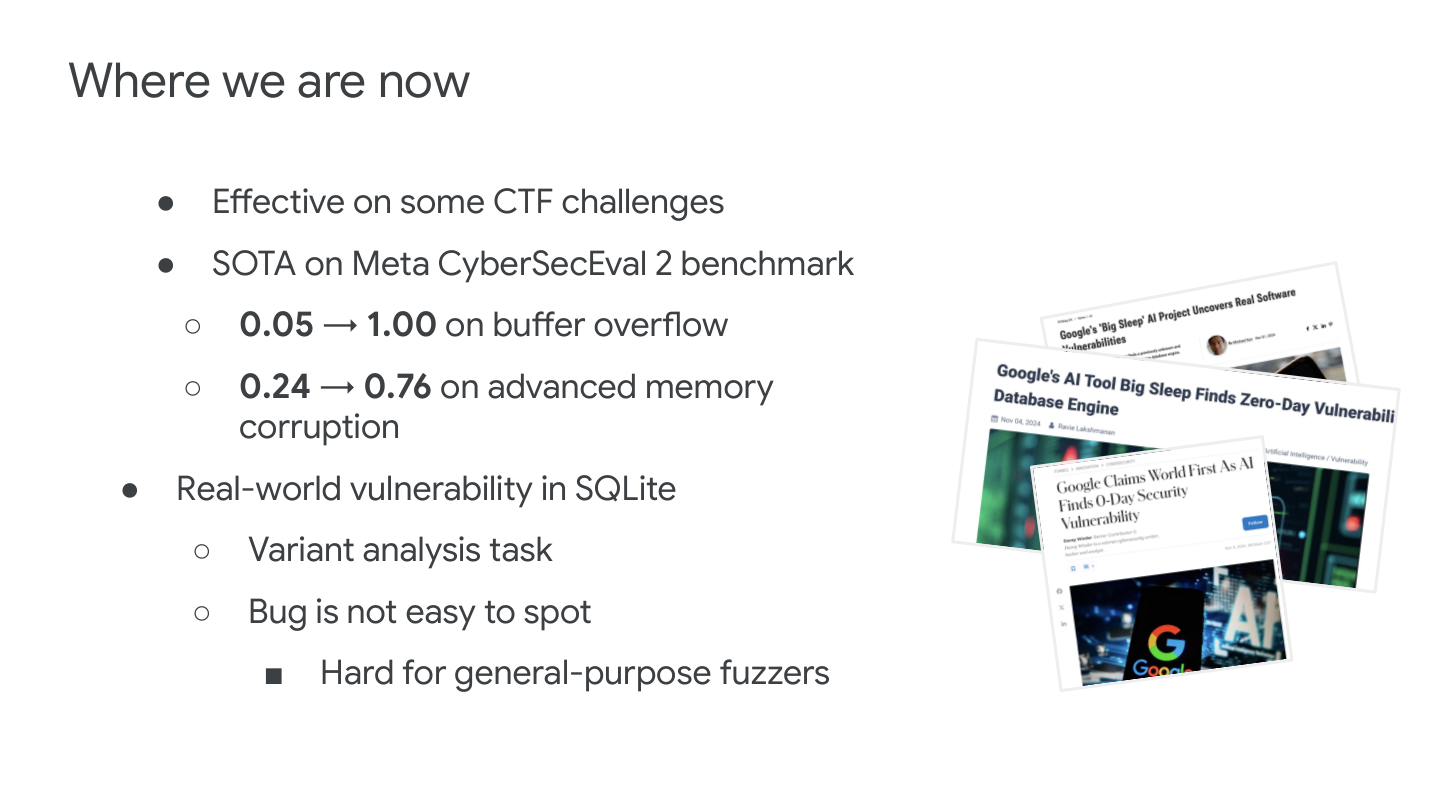
\includegraphics[width=0.82\textwidth]{../lectures/lec05_coding_agents_vulnerability_detection/figures/lec05_fig_008.png}
\caption{结果页体现的不是“模型更聪明”而是“workflow 更 grounded”：工具、验证和环境反馈让安全 agent 真正具备可交付价值。}
\end{figure}

\begin{warningbox}{安全 agent 的关键风险}
如果缺少 sandbox、工具权限约束、日志与 provenance 记录，security agent 可能同时变得不安全、不可审计，也无法复现实验结果。高风险任务中的 agent 设计，必须把 guardrails 当作一等公民。
\end{warningbox}

\section{与前后讲的关系、本章小结与复习}
本讲与 L04 的关系很直接：上一讲讨论 verifier 和 recipe，L05 则把这些思想带到 coding agents 和 vulnerability detection 中。系统不是靠“会说更复杂的 chain-of-thought”取胜，而是靠 evaluator、tool interface 和 environment feedback 形成闭环。

\section{本章小结}
本讲最重要的结论是：coding agents 的核心不是某个华丽 prompt，而是 control flow、工具接口和 evaluator 的共同设计。越到 security 这种高风险领域，越不能把“模型说得像”当成“系统真的对”；必须通过工具、执行和 verifier 建立 grounded workflow。

\section{复习题}
\begin{itemize}
\item 为什么 Sutton 把 evaluator 放在 coding-agent 设计的起点？
\item ReAct, Agentless, AutoCodeRover 在控制流上分别有什么差异？
\item 为什么 CTF/security tasks 更依赖 interactive tools？
\item 什么是 variant analysis，为什么它比开放式漏洞搜索更现实？
\item 为什么 security agent 必须把 sandbox 和 provenance 放进系统设计？
\end{itemize}

\section{深入思考题}
\begin{itemize}
\item 在什么 benchmark 条件下，dynamic agent 的优势会被 procedural pipeline 吃掉？
\item 安全 agent 的 verifier 应该如何设计，才能既减少误报又避免 reward hacking？
\item 如果给 Big Sleep 更多 test-time compute，应该优先加在 tool diversity、trajectory depth 还是 hypothesis generation 上？为什么？
\end{itemize}

\section{延伸阅读}
\begin{itemize}
\item EnIGMA: Interactive Tools Substantially Assist LM Agents in Finding Security Vulnerabilities
\item From Naptime to Big Sleep: Using Large Language Models To Catch Vulnerabilities In Real-World Code
\end{itemize}
